\documentclass{standalone}
\usepackage[dvipsnames]{xcolor}
\usepackage{tikz}

\begin{document}
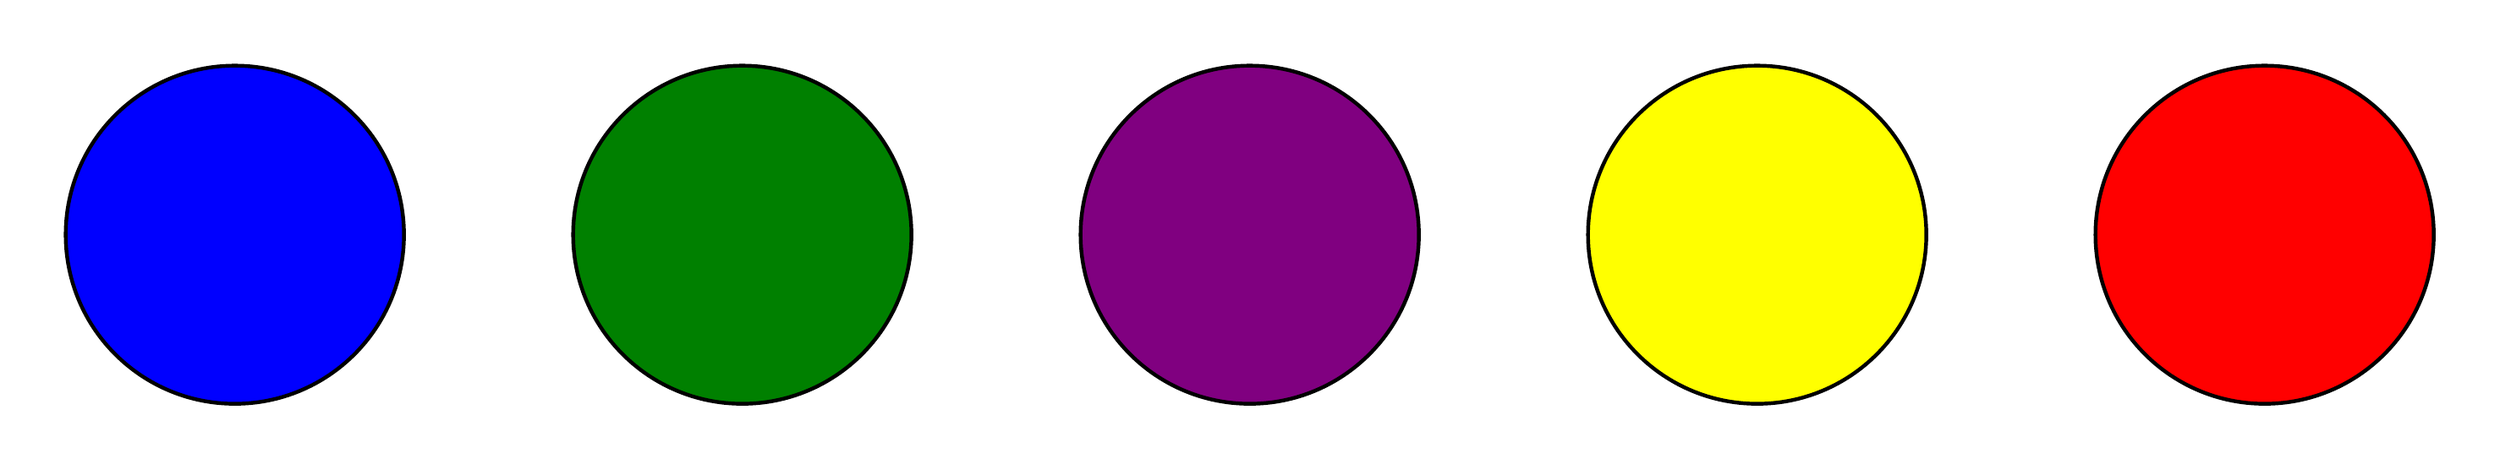
\begin{tikzpicture}[x=1in, y=1in]
	\node[draw, ultra thick, circle, minimum size=2in, inner sep=0pt, fill=Blue] at (0,0) {};
	\node[draw, ultra thick, circle, minimum size=2in, inner sep=0pt, fill=Green] at (3in,0) {};
	\node[draw, ultra thick, circle, minimum size=2in, inner sep=0pt, fill=Purple] at (6in,0) {};
	\node[draw, ultra thick, circle, minimum size=2in, inner sep=0pt, fill=Yellow] at (9in,0) {};
	\node[draw, ultra thick, circle, minimum size=2in, inner sep=0pt, fill=Red] at (12in,0) {};

\path (-1.25, -1.25) to (13.25,1.25);
\end{tikzpicture}
\end{document}